\vspace*{-5cm}
\chapter{Roboterbewegung im Occupancy Grid}
Die physikalische Umgebung des Roboters wird diskretisiert durch das \textit{Occupancy Grid}.
Dieser binäre, zweidimensionale Raum entspricht der Umgebung aus "Vogelperspektive". 

Das numpy Boolean Koordinatensystem \texttt{occupancy\_grid} mit der Länge \texttt{occupancy\_grid\_length} und Breite \texttt{occupancy\_grid\_width} hat den Ursprung links oben. Bedingt durch Numpy werden Koordinaten mit \texttt{occupancy\_grid[Y][X]} referenziert. Die Umgebung ist im Occupancy Grid binär, wodruch jede Koordinate ($X$,$Y$) durch ein Hindernis belegt ist (\texttt{occupancy\_grid[Y][X] == False}) oder frei von Hindernissen ist (\texttt{occupancy\_grid[Y][X] == True}).

\begin{figure}[h!]
	\small
	\centering	
	\begin{minipage}{0.46\textwidth}%
	\begin{minted}[
		obeytabs=true,
		tabsize=2,
		autogobble,
		fontsize={\fontsize{6.5}{8.5}\selectfont},
		frame=single
		]{python}
		occupancy_grid = 
		[[T, T, T, T, T, T, T, T, T, T, T, T, T, T, T, T, T, T, T, T],
		 [T, T, T, T, T, T, T, T, T, T, T, T, T, T, T, T, T, T, T, T],
		 [T, T, T, T, T, T, T, T, T, T, T, T, T, T, T, T, T, T, T, T],
		 [T, T, T, T, T, T, T, T, T, T, T, T, T, T, T, T, T, T, T, T],
		 [T, T, T, T, T, T, T, T, T, T, T, T, T, T, T, T, T, T, T, T],
		 [T, T, T, T, T, T, T, T, T, T, T, T, T, T, T, T, T, T, T, T],
		 [T, T, T, T, T, T, T, T, T, T, T, T, T, T, T, T, T, T, T, T],
		 [T, T, T, T, T, T, T, T, T, T, T, T, T, T, T, T, T, T, T, T],
		 [T, T, T, T, T, T, T, T, T, F, F, T, T, T, T, T, T, T, T, T],
		 [T, T, T, T, T, T, T, T, T, F, F, T, T, T, T, T, T, T, T, T],
		 [T, T, T, T, T, T, T, T, T, T, T, T, T, T, T, T, T, T, T, T],
		 [T, T, T, T, T, T, T, T, T, T, T, T, T, T, T, T, T, T, T, T],
		 [T, T, T, T, T, T, T, T, T, T, T, T, T, T, T, T, T, T, T, T],
		 [T, T, T, T, T, T, T, T, T, T, T, T, T, T, T, T, T, T, T, T],
		 [T, T, T, T, T, T, T, T, T, T, T, T, T, T, T, T, T, T, T, T],
		 [T, T, T, T, T, T, T, T, T, T, T, T, T, T, T, T, T, T, T, T],
		 [T, T, T, T, T, T, T, T, T, T, T, T, T, T, T, T, T, T, T, T],
		 [T, T, T, T, T, T, T, T, T, T, T, T, T, T, T, T, T, T, T, T],
		 [T, T, T, T, T, T, T, T, T, T, T, T, T, T, T, T, T, T, T, T]]
	\end{minted}
	\end{minipage}
	\hspace*{\fill}
	\begin{minipage}{0.46\textwidth}%
		\footnotesize
		\resizebox{\linewidth}{!}{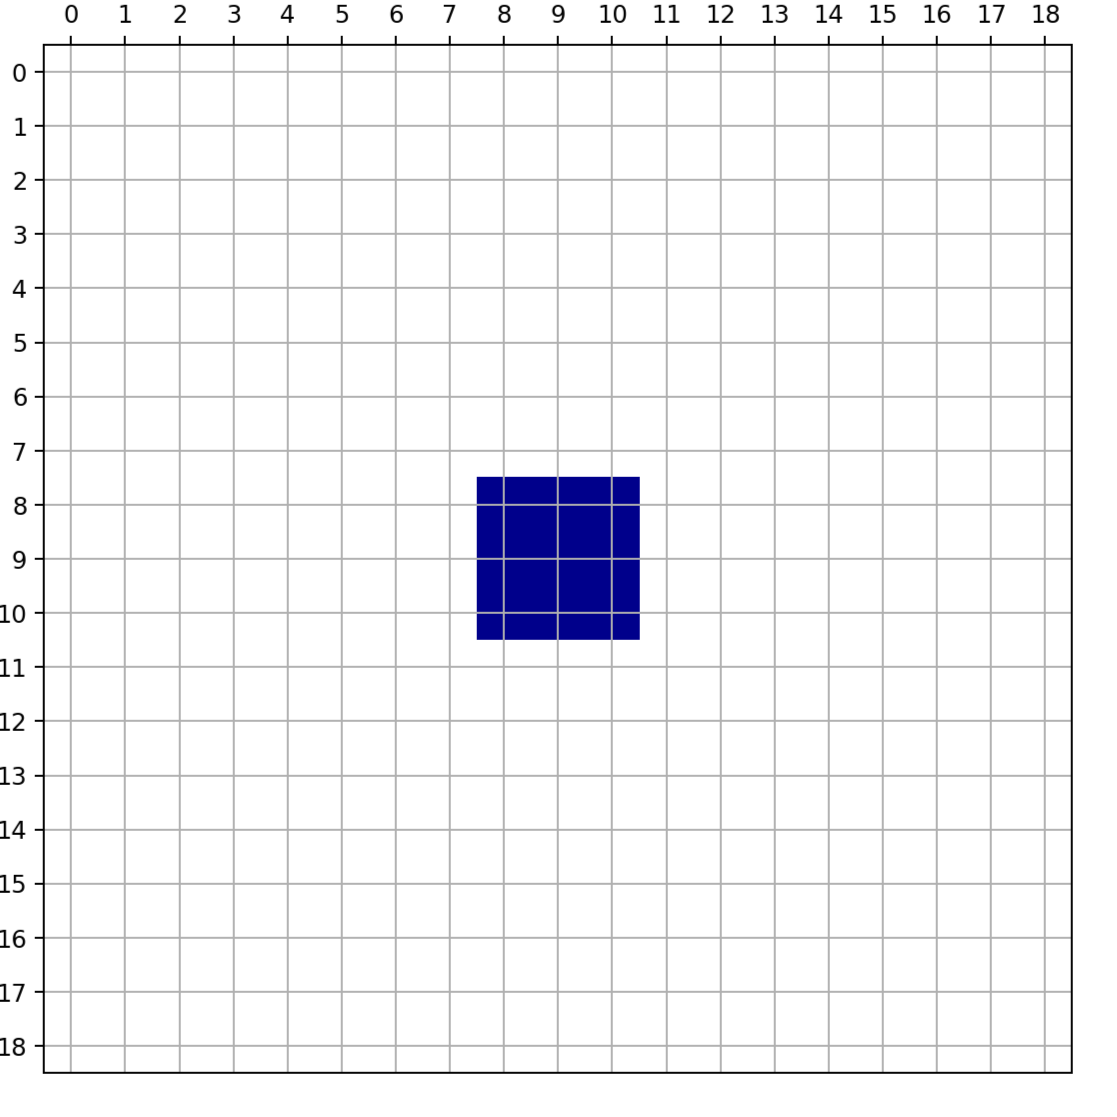
\includegraphics{bilder/occupancy-grid2.png}}
	\end{minipage}
	%	\vspace{-1cm}
	\caption{Im Occupancy Grid mit Ursprung links oben werden Hinderniskoordinaten mit \texttt{False} (\texttt{F}) markiert.}
\end{figure}

Gemäß der gestellten Anforderungen kann die Dimension des Roboters durch die Variablen \texttt{robot\_width} und \texttt{robot\_length} definiert werden. Pro Verarbeitungseinheit kann sich der Roboter entweder durch eine Translation oder Rotation im Occupancy Grid bewegen:
\begin{itemize}
\item \textbf{Translation} nach links (\texttt{x-1}), rechts (\texttt{x+1}), oben (\texttt{y-1}) und unten (\texttt{y+1})
\item \textbf{Rotation} um einen \textit{Ankerpunkt}. Bei einer Rotation von $0$° liegt dieser Referenzpunkt in der linken oberen Ecke des Roboters.
\end{itemize}

\begin{figure}[h!]
	\centering
	\small
	\centerline{\resizebox{\linewidth}{!}{\input{bilder/robotermodell_latex.pdf_tex}}}
	\caption{Translation (rechts) und Rotation (mitte) eines Roboters mit variablen Dimensionen (links).}
\end{figure}

*** TODO: Abbildung mit Roboter als Start- und Zielpunkt in Occupancy Grid ***